%!Mode::"UTF-8"
\documentclass[12pt]{article}

% 页面设置
\usepackage{geometry}
\geometry{left=2.5cm, right=2.5cm, top=2.5cm, bottom=2.5cm}
\usepackage{graphicx}
\usepackage{ctex}
\usepackage{fontspec}
\usepackage{setspace}

% 代码设置
\usepackage{listings}
\usepackage{color}
\setmonofont{Consolas}
\definecolor{listing}{gray}{0.97}
\lstset{
	backgroundcolor=\color{listing},
	basicstyle=\footnotesize,
	numbers=left,
	numberstyle=\footnotesize,
	stepnumber=1,
	aboveskip={0.5\baselineskip},
	belowskip={0.5\baselineskip},
	columns=fullflexible,
	breaklines=true,
	breakatwhitespace=true,
	frame=single,
	basicstyle=\ttfamily,
	numberstyle=\ttfamily,
	tabsize=2
}

% 字体设置
\setmainfont{Times New Roman}
\setCJKmainfont{SimSun}
\setCJKsansfont{SimHei}

% 表格设置
\usepackage{makecell}
\newcommand{\addcell}[2][4]{\makecell{\zihao{#1}\textsf{#2}}}
\usepackage{titlesec}
\usepackage{booktabs}
\usepackage{tabularx}

% 设置图注、表注
\usepackage{caption}
\usepackage{bicaption}
\captionsetup{labelsep=quad, font={small, bf}, skip=2pt}
\DeclareCaptionOption{english}[]{
    \renewcommand\figurename{Fig.}
    \renewcommand\tablename{Table}
}
\captionsetup[bi-second]{english}

% 设置页眉
\usepackage{fancyhdr}
\pagestyle{fancy}
\fancypagestyle{preContent}{
    \fancyhead[L]{\zihao{-5} 物理化学实验}
    \fancyhead[C]{\zihao{-5} 实验八\ \ 铂电极表面的电化学反应}
    \fancyhead[R]{\zihao{-5} 1800011828\ 王宇哲}
}
\pagestyle{preContent}

%	设置首页页眉页脚
\fancypagestyle{plain}{
	\fancyhead[L]{\zihao{-5} 物理化学实验}
	\fancyhead[C]{\zihao{-5} 实验八\ \ 铂电极表面的电化学反应}
	\fancyhead[R]{\zihao{-5} 1800011828\ 王宇哲}
	\cfoot{}
}

% 设置标题格式
\titleformat*{\section}{\zihao{4}\sffamily}
\titleformat*{\subsection}{\zihao{-4}\sffamily}
\titleformat*{\subsubsection}{\zihao{-4}\sffamily}
\titlespacing*{\section}{0pt}{10pt}{10pt}
\titlespacing*{\subsection}{0pt}{10pt}{5pt}
\titlespacing*{\subsubsection}{0pt}{10pt}{5pt}

% 设置引用格式
\usepackage[super,round,comma,compress]{natbib}

\usepackage{amsmath}
\usepackage{amssymb}

%设置封面
\begin{document}
    % 标题页
    \begin{titlepage}
    	% 页眉
    	\thispagestyle{plain}
        % 图片
        \begin{figure}[h]
            \centering
            \includegraphics{pku.png}
        \end{figure}
        \vspace{24pt}
        % 标题
        \centerline{\zihao{-0} \textsf{物理化学实验报告}}
        \vspace{40pt} % 空行
        \begin{center}
            \begin{tabular}{cp{9.5 cm}}
                % 题目
                \addcell[2]{题目:\ } & \addcell[2]{铂电极表面的电化学反应} \\
                \cline{2-2}
            \end{tabular}
        \end{center}
        \vspace{20pt} % 空行
        \begin{center}
            \doublespacing
            \begin{tabular}{cp{5cm}}
                % 姓名
                \addcell{姓\phantom{空格}名:\ } & \addcell{王宇哲} \\
                \cline{2-2}
                % 学号
                \addcell{学\phantom{空格}号:\ } & \addcell{1800011828}\\
                \cline{2-2}
                % 组别
                \addcell{组\phantom{空格}别:\ } & \addcell{11组} \\
                \cline{2-2}
                % 实验日期
                \addcell{实验日期:\ } & \addcell{2020.11.18}\\
                \cline{2-2}
                % 室温
                \addcell{室\phantom{空格}温:\ } & \addcell{291.35\ K}\\
                \cline{2-2}
                % 大气压强
                \addcell{大气压强:\ } & \addcell{100.72\ kPa}\\
                \cline{2-2}
            \end{tabular}
            \begin{tabular*}{\textwidth}{c}
                \\ % 这是空行
                \\ % 这是空行
                \\ % 这是空行
                \\ % 这是空行
                \hline % 分割线
            \end{tabular*}
        \end{center}
        % 摘要
        \textsf{摘\ \ 要}\ \ 本实验使用三电极电解池研究铂电极表面的电化学反应,用${\rm N_{2}}$饱和的${\rm 0.05 \ \ M}$硫酸对电极系统进行活化,测定了扫描速度为$0.5$、$0.2$和$0.1\ \ {\rm V\cdot s^{-1}}$时的CV曲线,对CV曲线进行积分,得到铂电极电化学活性面积$S=0.016\ \ {\rm cm^{2}}$。测定了不同搅拌速度下铂电极表面氧还原反应的CV曲线,读出氧气的起始还原电位$0.57\ \ {\rm V}$。测定铂电极表面甲醇氧化反应的CV曲线,读出甲醇的起始氧化电位$0.06\ \ {\rm V}$。绘制了直接甲醇燃料电池的$U-P$曲线,工作电压为$0.2\ \ {\rm V}$时达到最大输出功率$3.5\times 10^{-7}\ \ {\rm W}$。
        \\
        \\
        % 关键字
        \textsf{关键词}\ \ 循环伏安法;直接甲醇燃料电池;电化学活性面积;电极极化
    \end{titlepage}

    \section{引言}
	略
               
\vbox{}        
    \section{实验部分}
    	\subsection{仪器和药品}
    	\subsubsection{仪器}
    	三电极电解池,工作电极(W.E.)为铂圆盘电极,辅助电极(C.E.)采用铂片电极,参比电极(R.E.)使用双盐桥饱和甘汞电极。\par 
    	CHI电化学工作站,磁力搅拌恒温槽,温度计,氧气钢瓶,氮气钢瓶。
    	\subsubsection{试剂}
    	电解质:$0.05\ \ {\rm M}$硫酸水溶液,$0.1\ \ {\rm M}$硫酸水溶液,$0.1\ \ {\rm M}$甲醇水溶液。去离子水。
\vbox{}
    	 \subsection{实验内容\citealp{physchemlab}}
			\subsubsection{电极的清洗及组装}
用去离子水清洗电极系统和电解池,向参比电极的二次盐桥与电解池中加入适量$0.05 \ \ {\rm M}$硫酸溶液。\par 
将三电极电解池与CHI电化学工作站相连:工作电极铂圆盘电极与绿线相连,辅助电极铂片电极与红线相连,参比电极双盐桥饱和甘汞电极与白线相连。通入$\rm N_{2}$赶走电解质溶液中的残余$\rm O_{2}$直至饱和。
\subsubsection{$0.05 \ \ {\rm M}$硫酸溶液中的测试}
调整电位窗口,使得在电位窗口内水不发生电解,同时包含所要研究的电化学信息,确定电位窗口为$-0.28\sim 1.15\ \ {\rm V}$。在确定的电位窗口内用CV法活化电极,以$0.5\ \ {\rm V\cdot s^{-1}}$的扫速扫描$500$个周期,观察CV曲线形状基本保持不变后停止活化。\par 
在$\rm N_{2}$饱和下测量CV,测定不同扫描速度$0.5\ \ {\rm V\cdot s^{-1}}$、$0.2\ \ {\rm V\cdot s^{-1}}$、$0.1\ \ {\rm V\cdot s^{-1}}$下的CV曲线。
			\subsubsection{铂电极表面的氧还原反应}
向电解池内通入$\rm O_{2}$至饱和,设定扫描速度为$0.1\ \ {\rm V\cdot s^{-1}}$,考察不同搅拌速度对氧还原反应的影响,分别测定快速搅拌(通气并开搅拌)、低速搅拌(停搅拌仅通气)、电解质静止(停搅拌不通气)条件下的CV曲线。
			\subsubsection{铂电极表面的甲醇电化学氧化反应}
将$0.1\ \ {\rm M}$硫酸水溶液与$0.1\ \ {\rm M}$甲醇水溶液等体积混合加入电解池,通入$\rm N_{2}$排除溶液中残余的空气,设定扫描速度为$0.1\ \ {\rm V\cdot s^{-1}}$,测定CV曲线。
	\subsubsection{清洁电解池和电极}
用去离子水清洗电解池和电极,测量$\rm N_{2}$氛围下$0.05\ \ {\rm M}$硫酸溶液中的CV曲线,与实验开始时相同条件测量的曲线一致后,将实验仪器复原到初始状态。
\vbox{}
 \section{数据与结果}
 \subsection{实验数据记录及处理}
 \subsubsection{$0.05\ \ {\rm M}$硫酸溶液中的测试}
 测定不同扫描速度下的CV曲线,为便于观察仅示出第$9\sim 10$个segment,结果如\textbf{图1}所示,图中Empty05(红色曲线)、Empty02(蓝色曲线)、Empty01(棕色曲线)分别为$0.5\ \ {\rm V\cdot s^{-1}}$、$0.2\ \ {\rm V\cdot s^{-1}}$、$0.1\ \ {\rm V\cdot s^{-1}}$下的CV曲线。
 \begin{figure}[h]
 	\centering
 	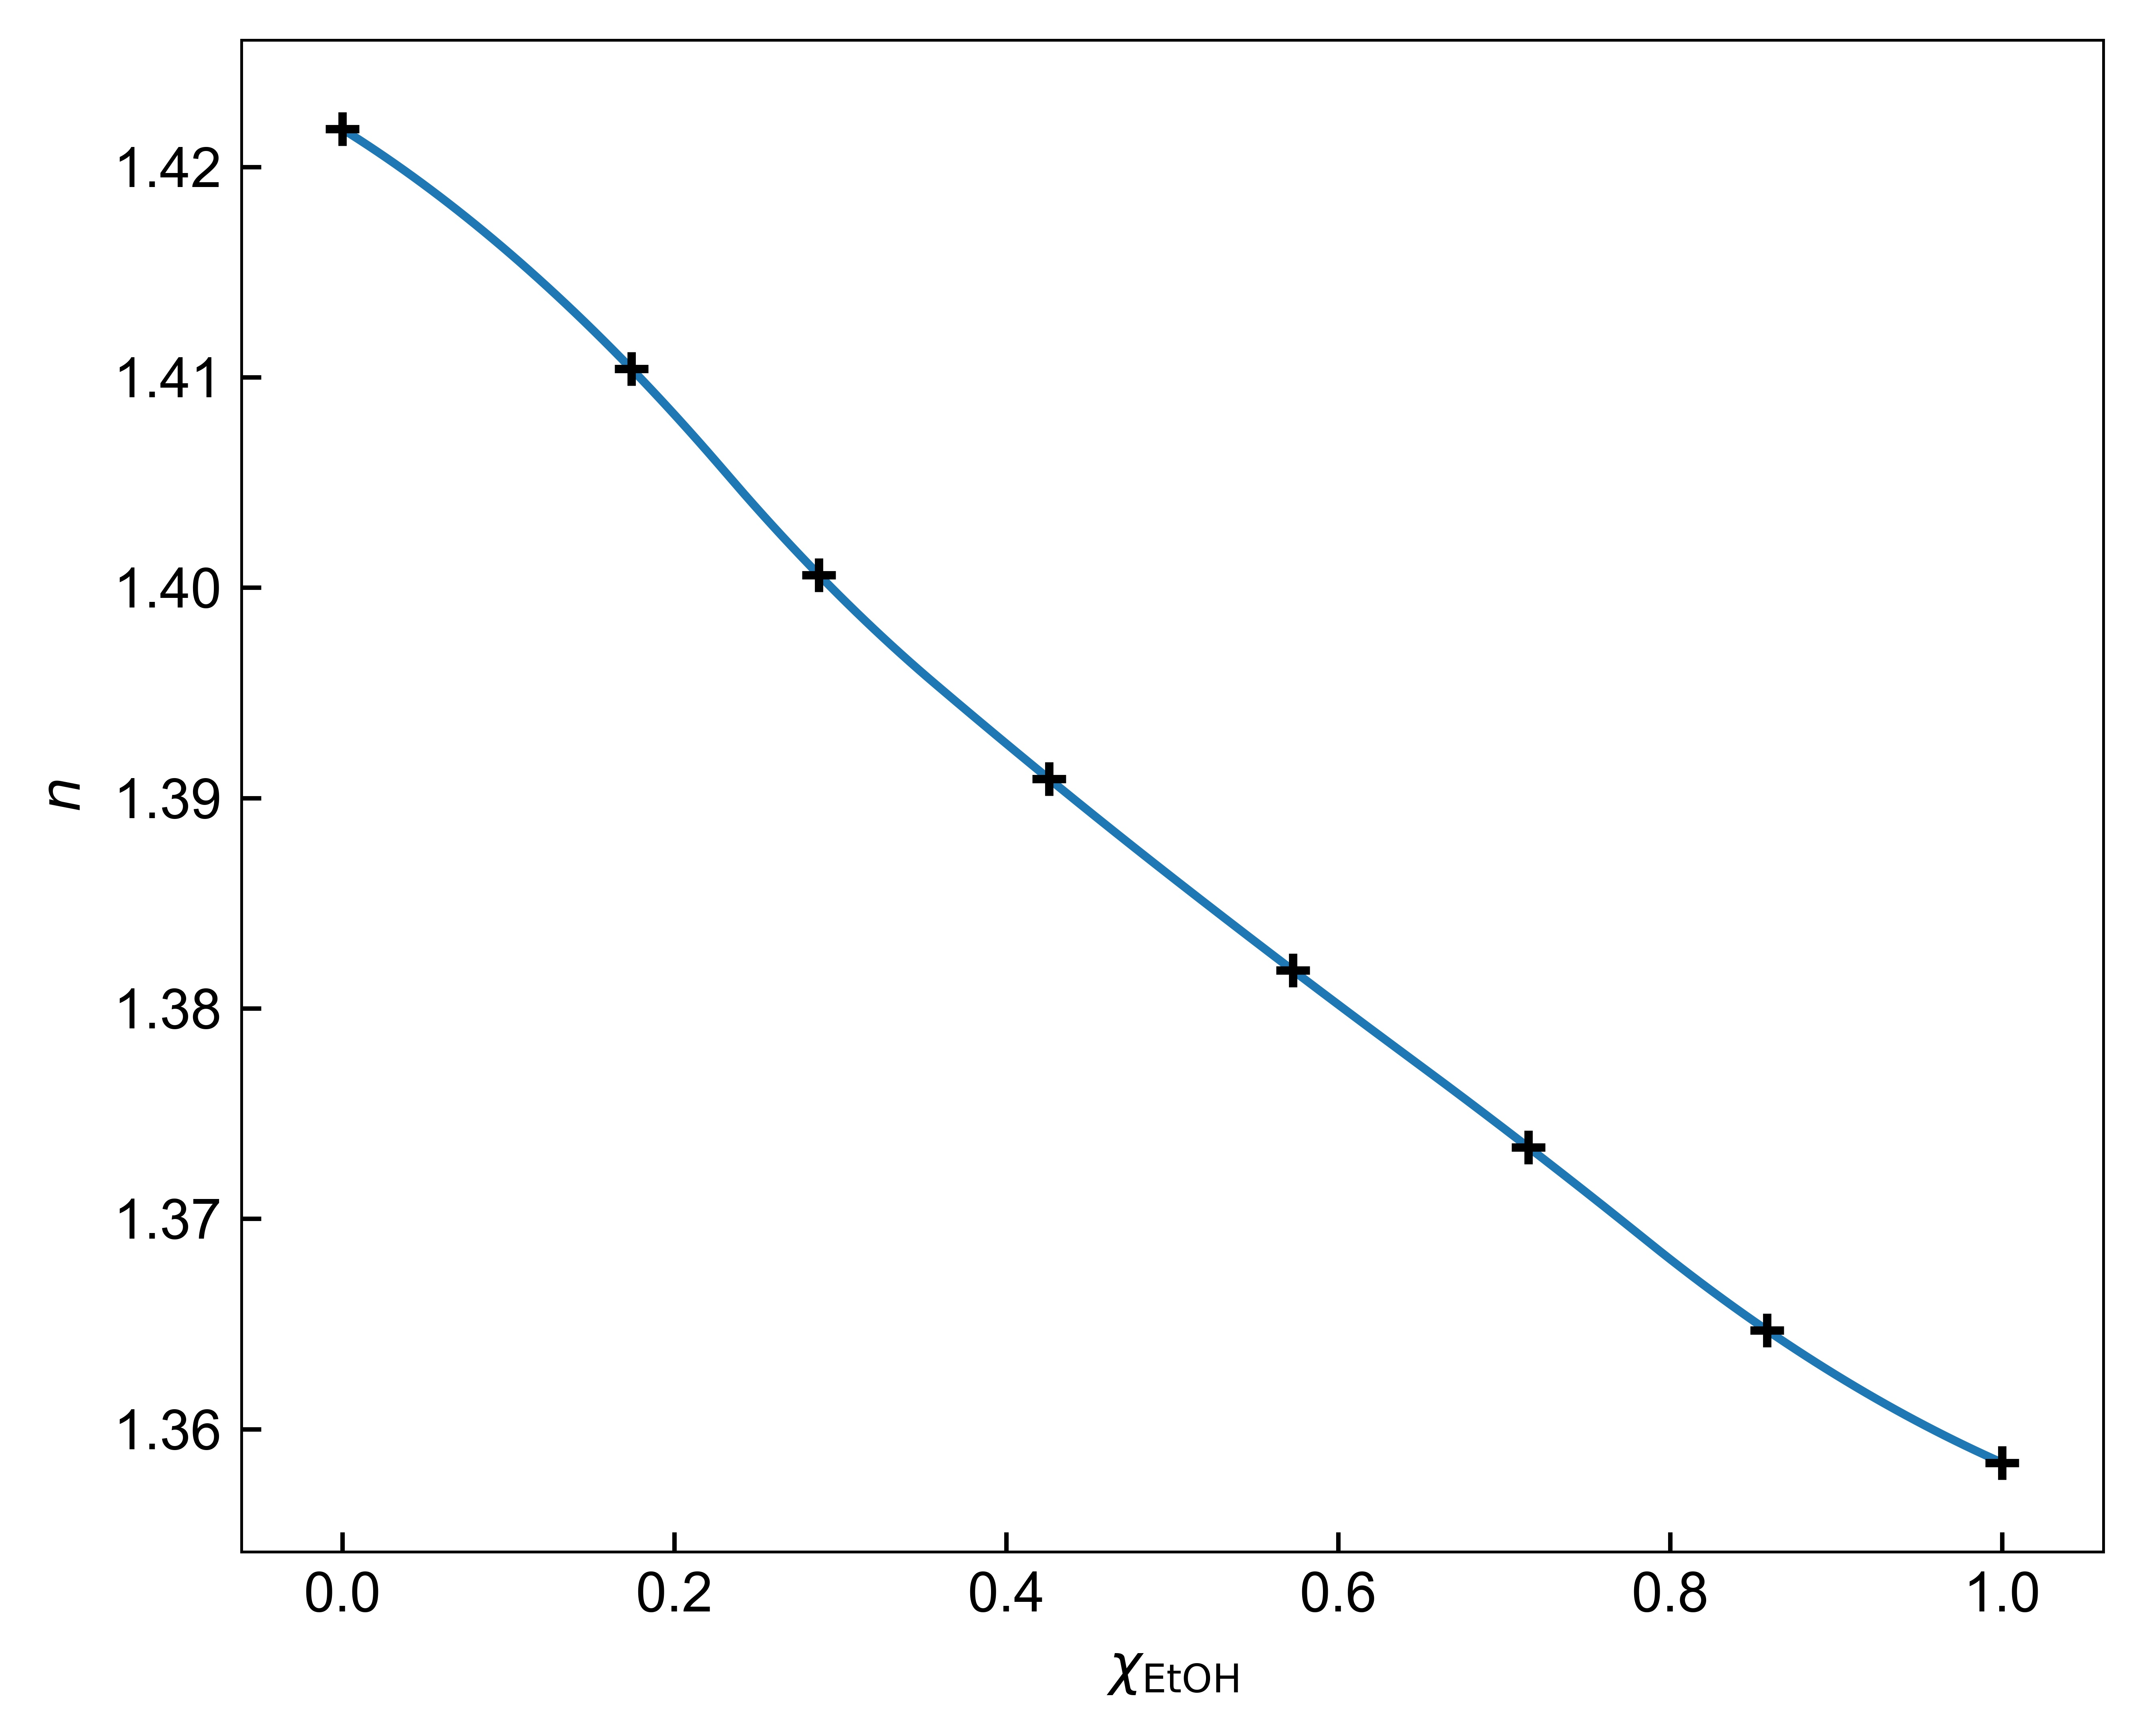
\includegraphics[width=0.7\textwidth]{1.bmp}
 	\bicaption{不同扫描速度下的CV曲线}{CV curve under different scanning speed}
 \end{figure}
 \par
 从\textbf{图1}可以看出,不同扫描速度下,峰电位位置基本不变,但扫描速度越大峰电流越大,这与循环伏安法的原理是相符的。根据Randles–Ševčík方程,峰电流$i_{p}$满足
 $$
 i_{p}=0.4463 n F A C\sqrt{\frac{nFvD}{RT}}\propto\sqrt{v}
 $$
$v$为扫描速度。因此,峰电流$i_{p}$随扫描速度$v$的增大而增大,这与观察到的实验现象一致。
\subsubsection{铂电极表面的氧还原反应}
测定不同搅拌速度下氧还原反应的CV曲线,为便于观察仅示出1个segment(即为线性扫描曲线LSV),结果如\textbf{图2}所示,图中O2a(棕色曲线)、O2b(红色曲线)、O2c(蓝色曲线)分别为快速搅拌、低速搅拌、电解质静止下的LSV曲线。
\begin{figure}[h]
	\centering
	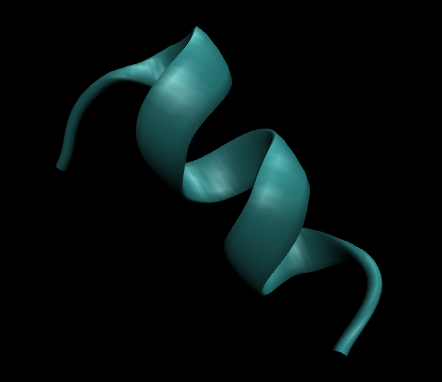
\includegraphics[width=0.7\textwidth]{2.bmp}
	\bicaption{不同搅拌速度下氧还原反应的LSV曲线}{LSV curve of oxygen reduction reaction under different stirring speed}
\end{figure}
\par
从\textbf{图2}可以看出,不同搅拌速度下氧还原反应的LSV曲线走势大致相同,对于不涉及氧还原反应的部分(电势高于$\sim0.4{\rm V}$),不同搅拌速度下的LSV曲线基本重合;而对于电势较低的氧还原电势区(电势低于$\sim 0.4{\rm V}$),搅拌越剧烈,氧还原的峰电流$i_{p}$越大,并且LSV曲线的波动越显著;这是由于在搅拌速度较快时,物质传输速度快,铂电极附近消耗的$\rm O_{2}$和$\rm H^{+}$能得到及时补充,浓度更大,因此氧还原的峰电流$i_{p}$较大;但由于搅拌速度较快时对铂电极附近溶液产生较大扰动,$\rm O_{2}$、$\rm H^{+}$浓度变化剧烈,导致LSV曲线产生显著波动。\par 
对比扫描速度为$0.1\ \ {\rm V\cdot s^{-1}}$、$\rm N_{2}$饱和的硫酸溶液中铂电极的CV曲线和扫描速度为$0.1\ \ {\rm V\cdot s^{-1}}$、电解质静止、$\rm O_{2}$饱和的硫酸溶液中氧还原反应的CV曲线,为便于观察仅示出第$9\sim 10$个segment,如\textbf{图3}所示,图中Empty01(红色曲线)、O2full(蓝色曲线)分别为氮气饱和与氧气饱和的硫酸溶液中的CV曲线。
\begin{figure}[h]
	\centering
	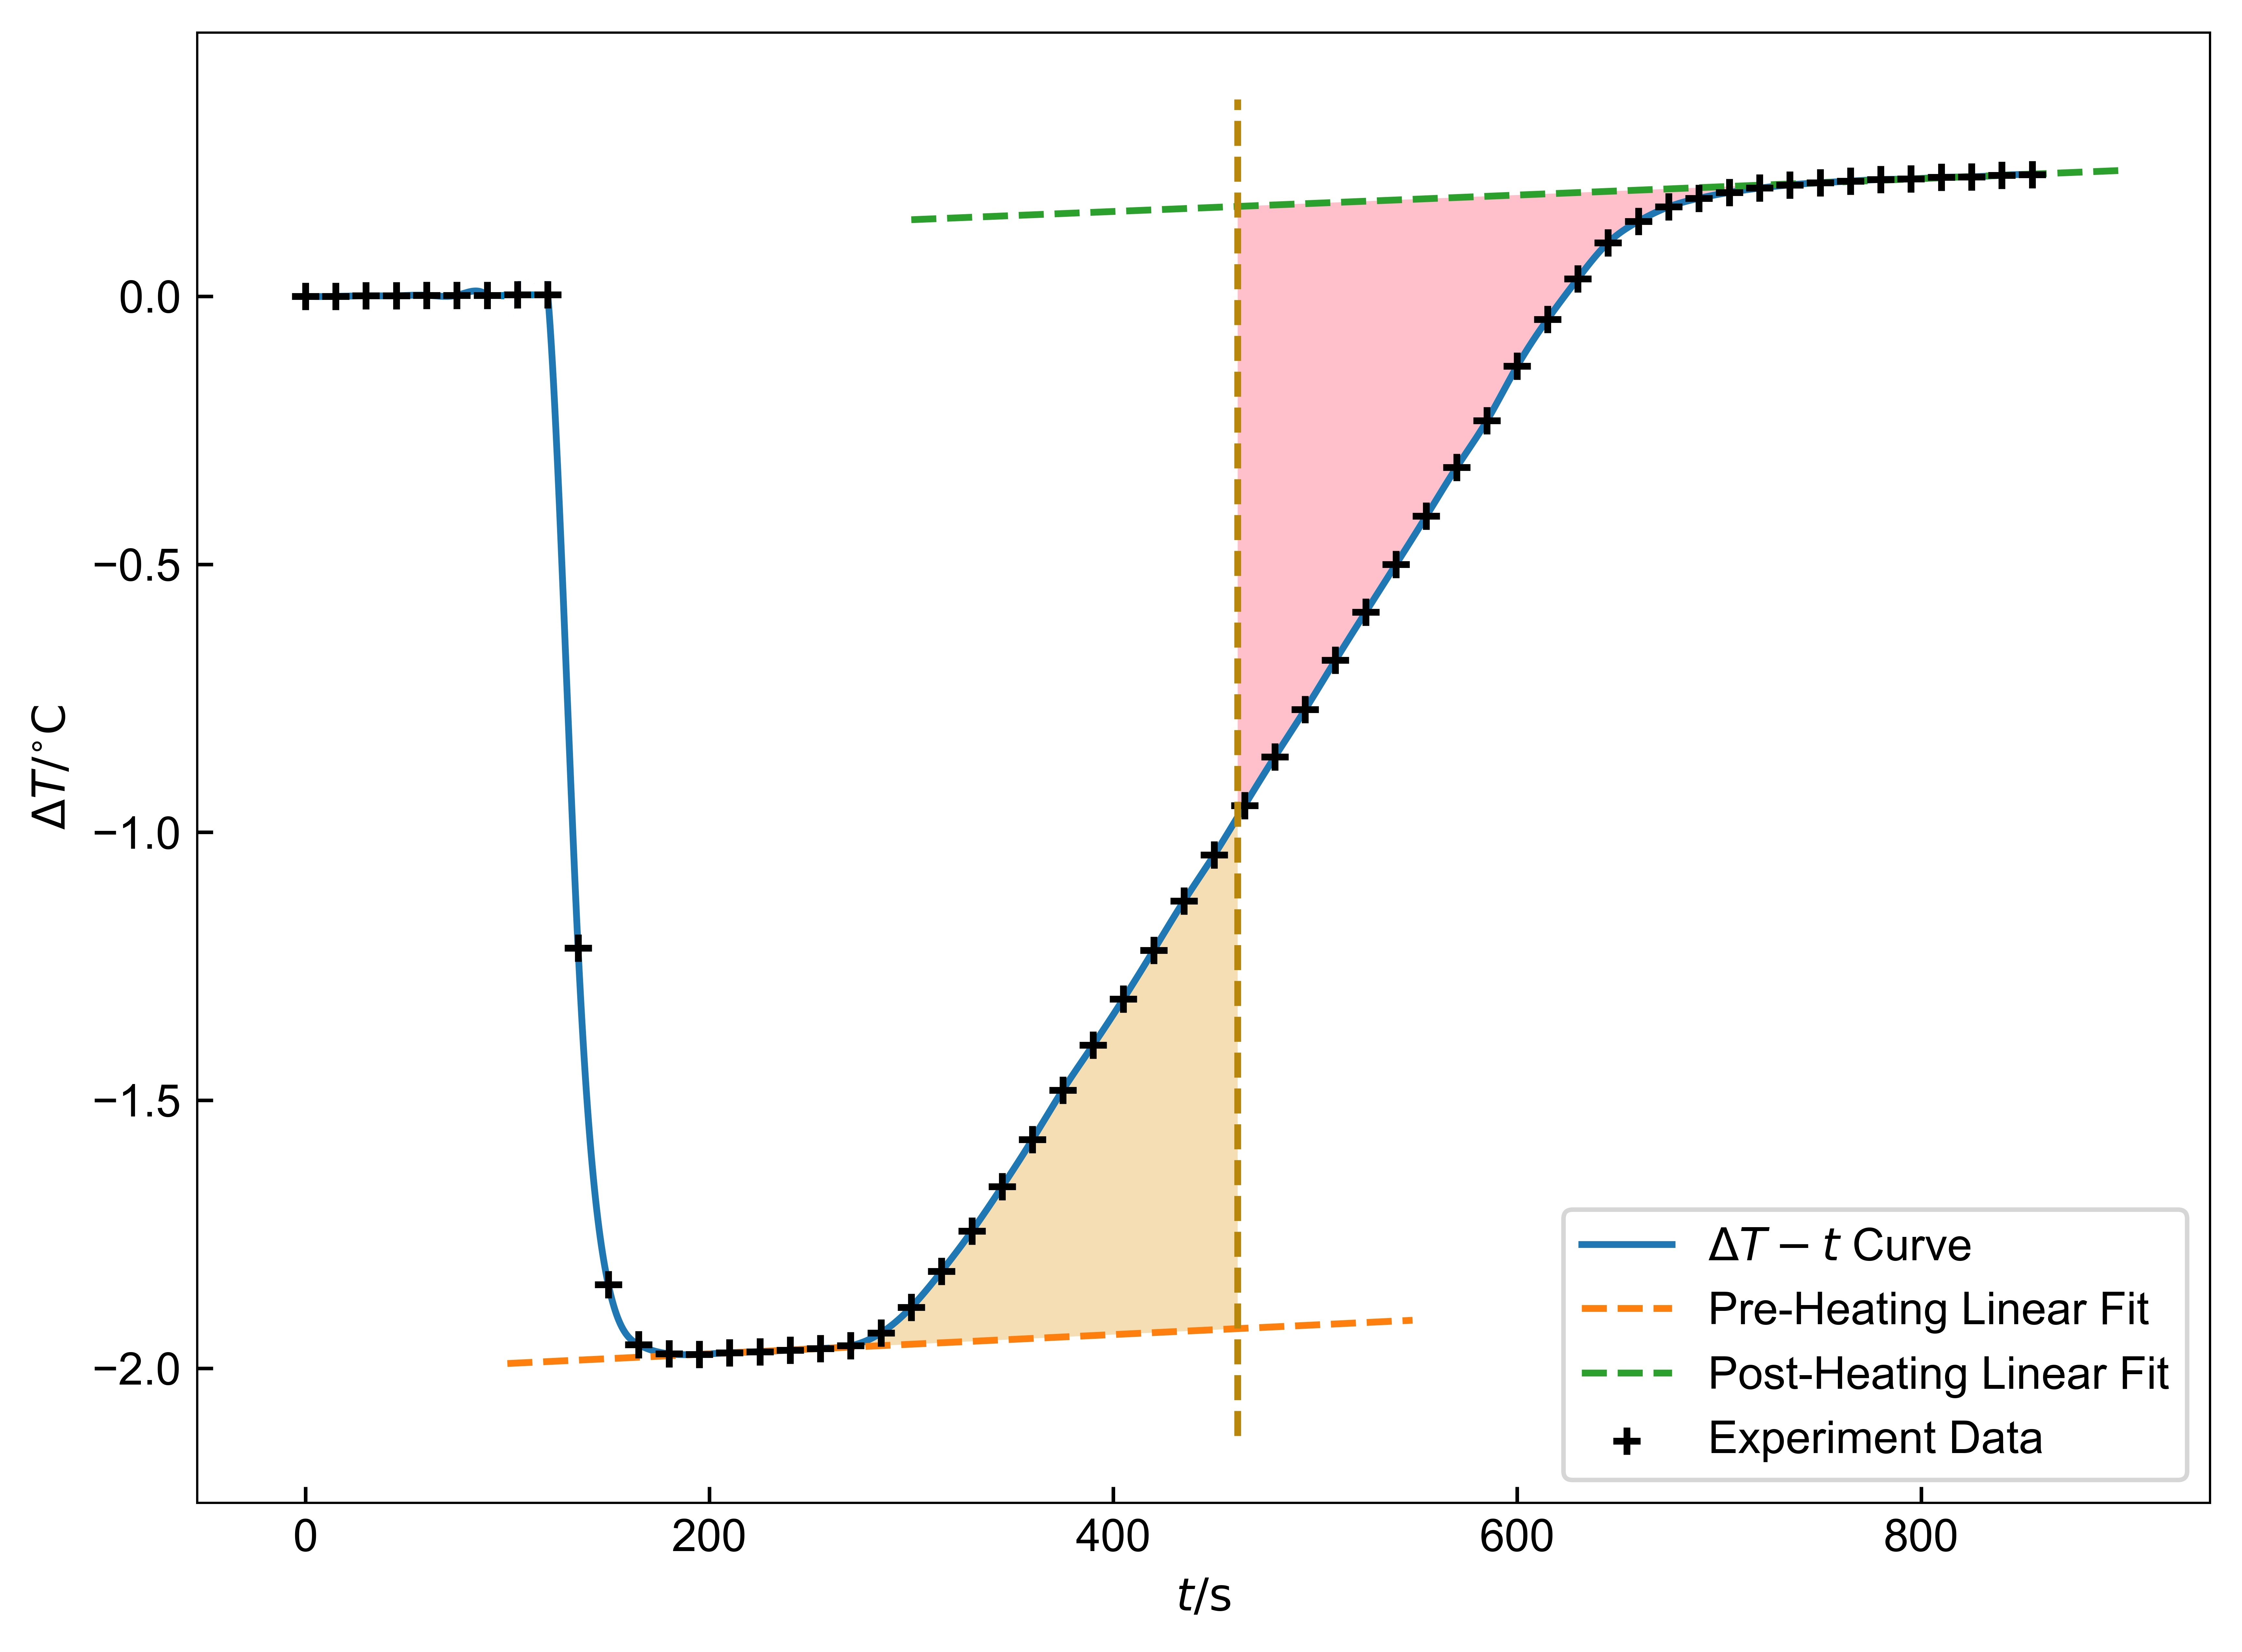
\includegraphics[width=0.7\textwidth]{3.bmp}
	\bicaption{氮气与氧气饱和的硫酸溶液中的CV曲线}{CV curve in sulfuric acid solution saturated with nitrogen and oxygen}
\end{figure}
\par
根据\textbf{图3},读出电势升高过程中含氧物种吸附氧化的起始氧化电位为$0.66\ \ {\rm V}$,电势降低过程中氧气的起始还原电位为$0.57\ \ {\rm V}$。故若以起始还原电位为基准,氧化过程中氧的过电势
$$
\eta_{\rm O}=(0.66-0.57)\ \ {\rm V}=0.11\ \ {\rm V}
$$
推测该过电势$\eta_{\rm O}$的形成是由于含氧物种吸附氧化过程中,氧气在铂电极表面析出的电化学反应迟缓,造成了电化学极化,从而导致电势升高和电势降低过程中氧气的起始氧化电位和起始还原电位不相等。
\subsubsection{铂电极表面的甲醇电化学氧化反应}
测定铂电极表面甲醇电化学氧化反应的CV曲线,为便于观察仅示出第$9\sim 10$个segment,结果如\textbf{图4}所示,图中MeOH(红色曲线)、Empty01(蓝色曲线)分别为硫酸溶液中铂电极表面甲醇电化学氧化与氮气饱和的CV曲线。
\begin{figure}[h]
	\centering
	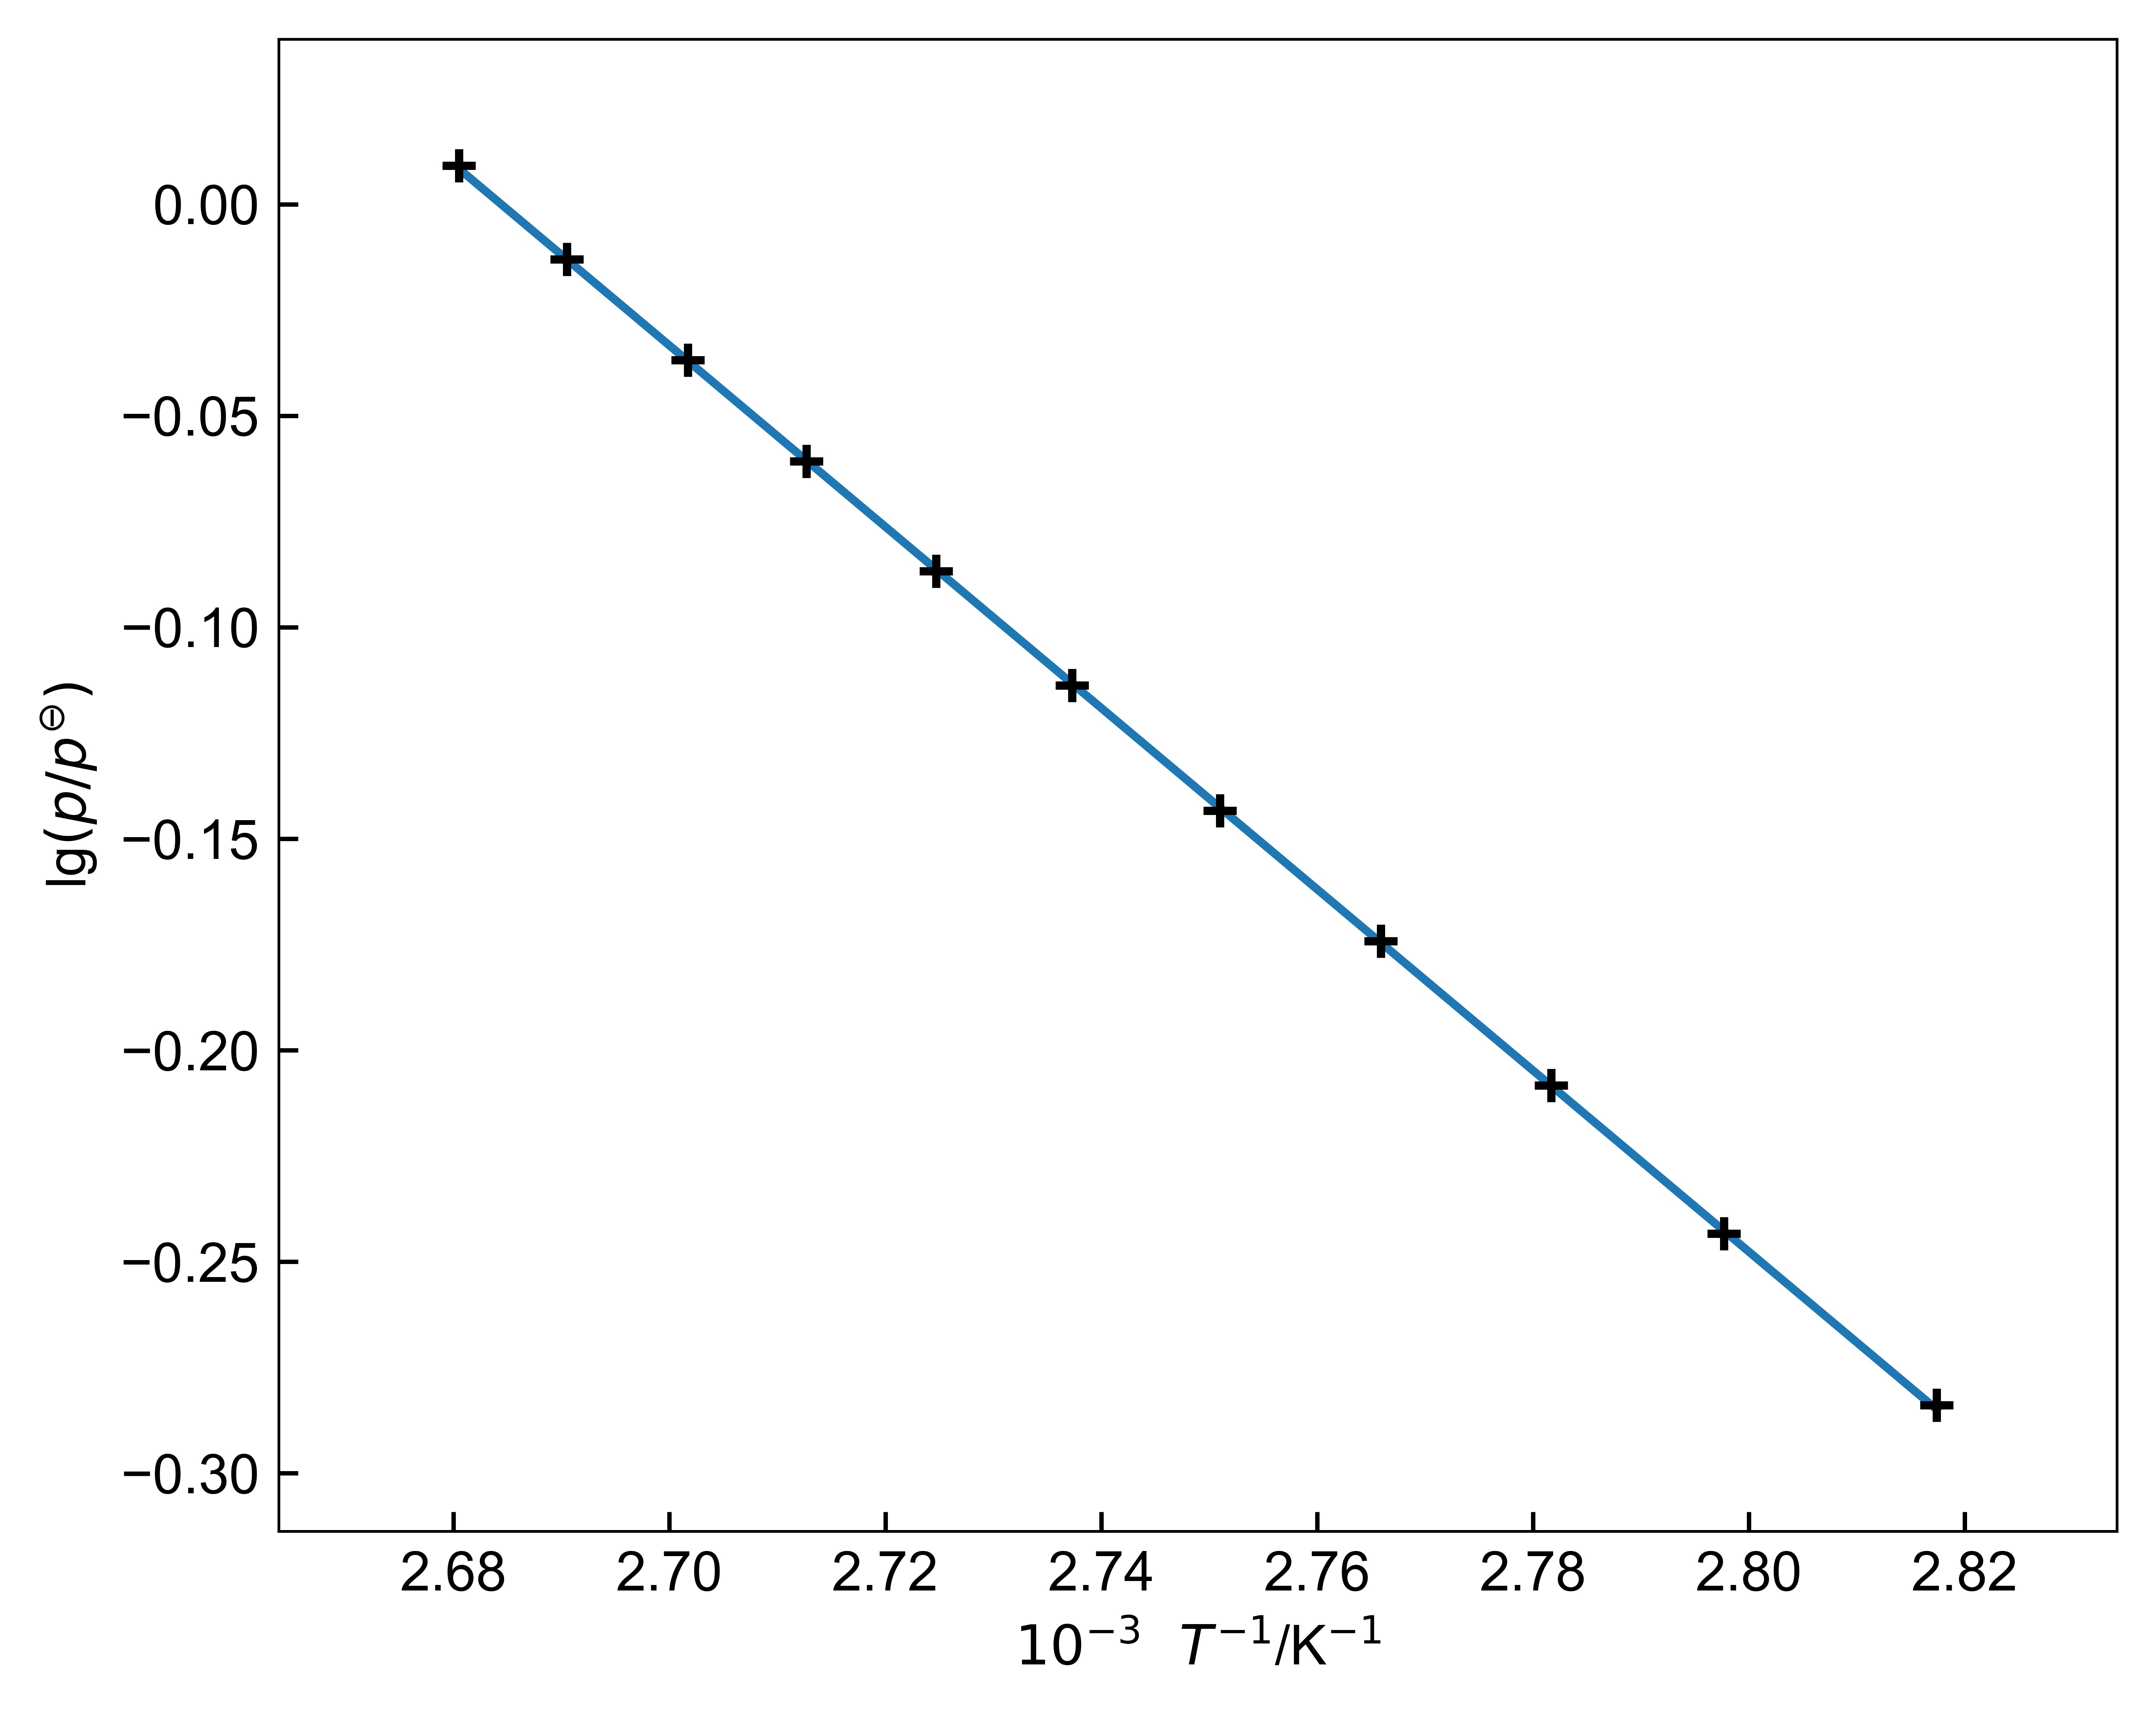
\includegraphics[width=0.7\textwidth]{4.bmp}
	\bicaption{硫酸溶液中甲醇氧化与氮气饱和的CV曲线}{CV curve of methanol oxidation and nitrogen saturation in sulfuric acid solution}
\end{figure}
\par
根据\textbf{图4},读出甲醇的起始氧化电位为$0.06\ \ {\rm V}$。

 \subsection{数据处理结果与分析}
 \subsubsection{铂电极的电化学活性面积}
 利用氮气饱和的硫酸溶液中铂电极的CV曲线中氢原子脱附峰的电量求算铂电极的电化学活性面积。取扫描速度为$0.1\ \ {\rm V\cdot s^{-1}}$下的CV曲线第9个segment的实验数据,根据扫描速度,将原始数据的横坐标电势$\varphi$换算成时间$t$,以双电层电位作为基线,使用Origin对氢原子脱附峰峰面积进行积分,得到氢原子脱附峰的电量,结果如\textbf{图5}所示,图中红色直线即为双电层电位基线,Area为积分面积,FWHM为半峰宽。
 \begin{figure}[h]
 	\centering
 	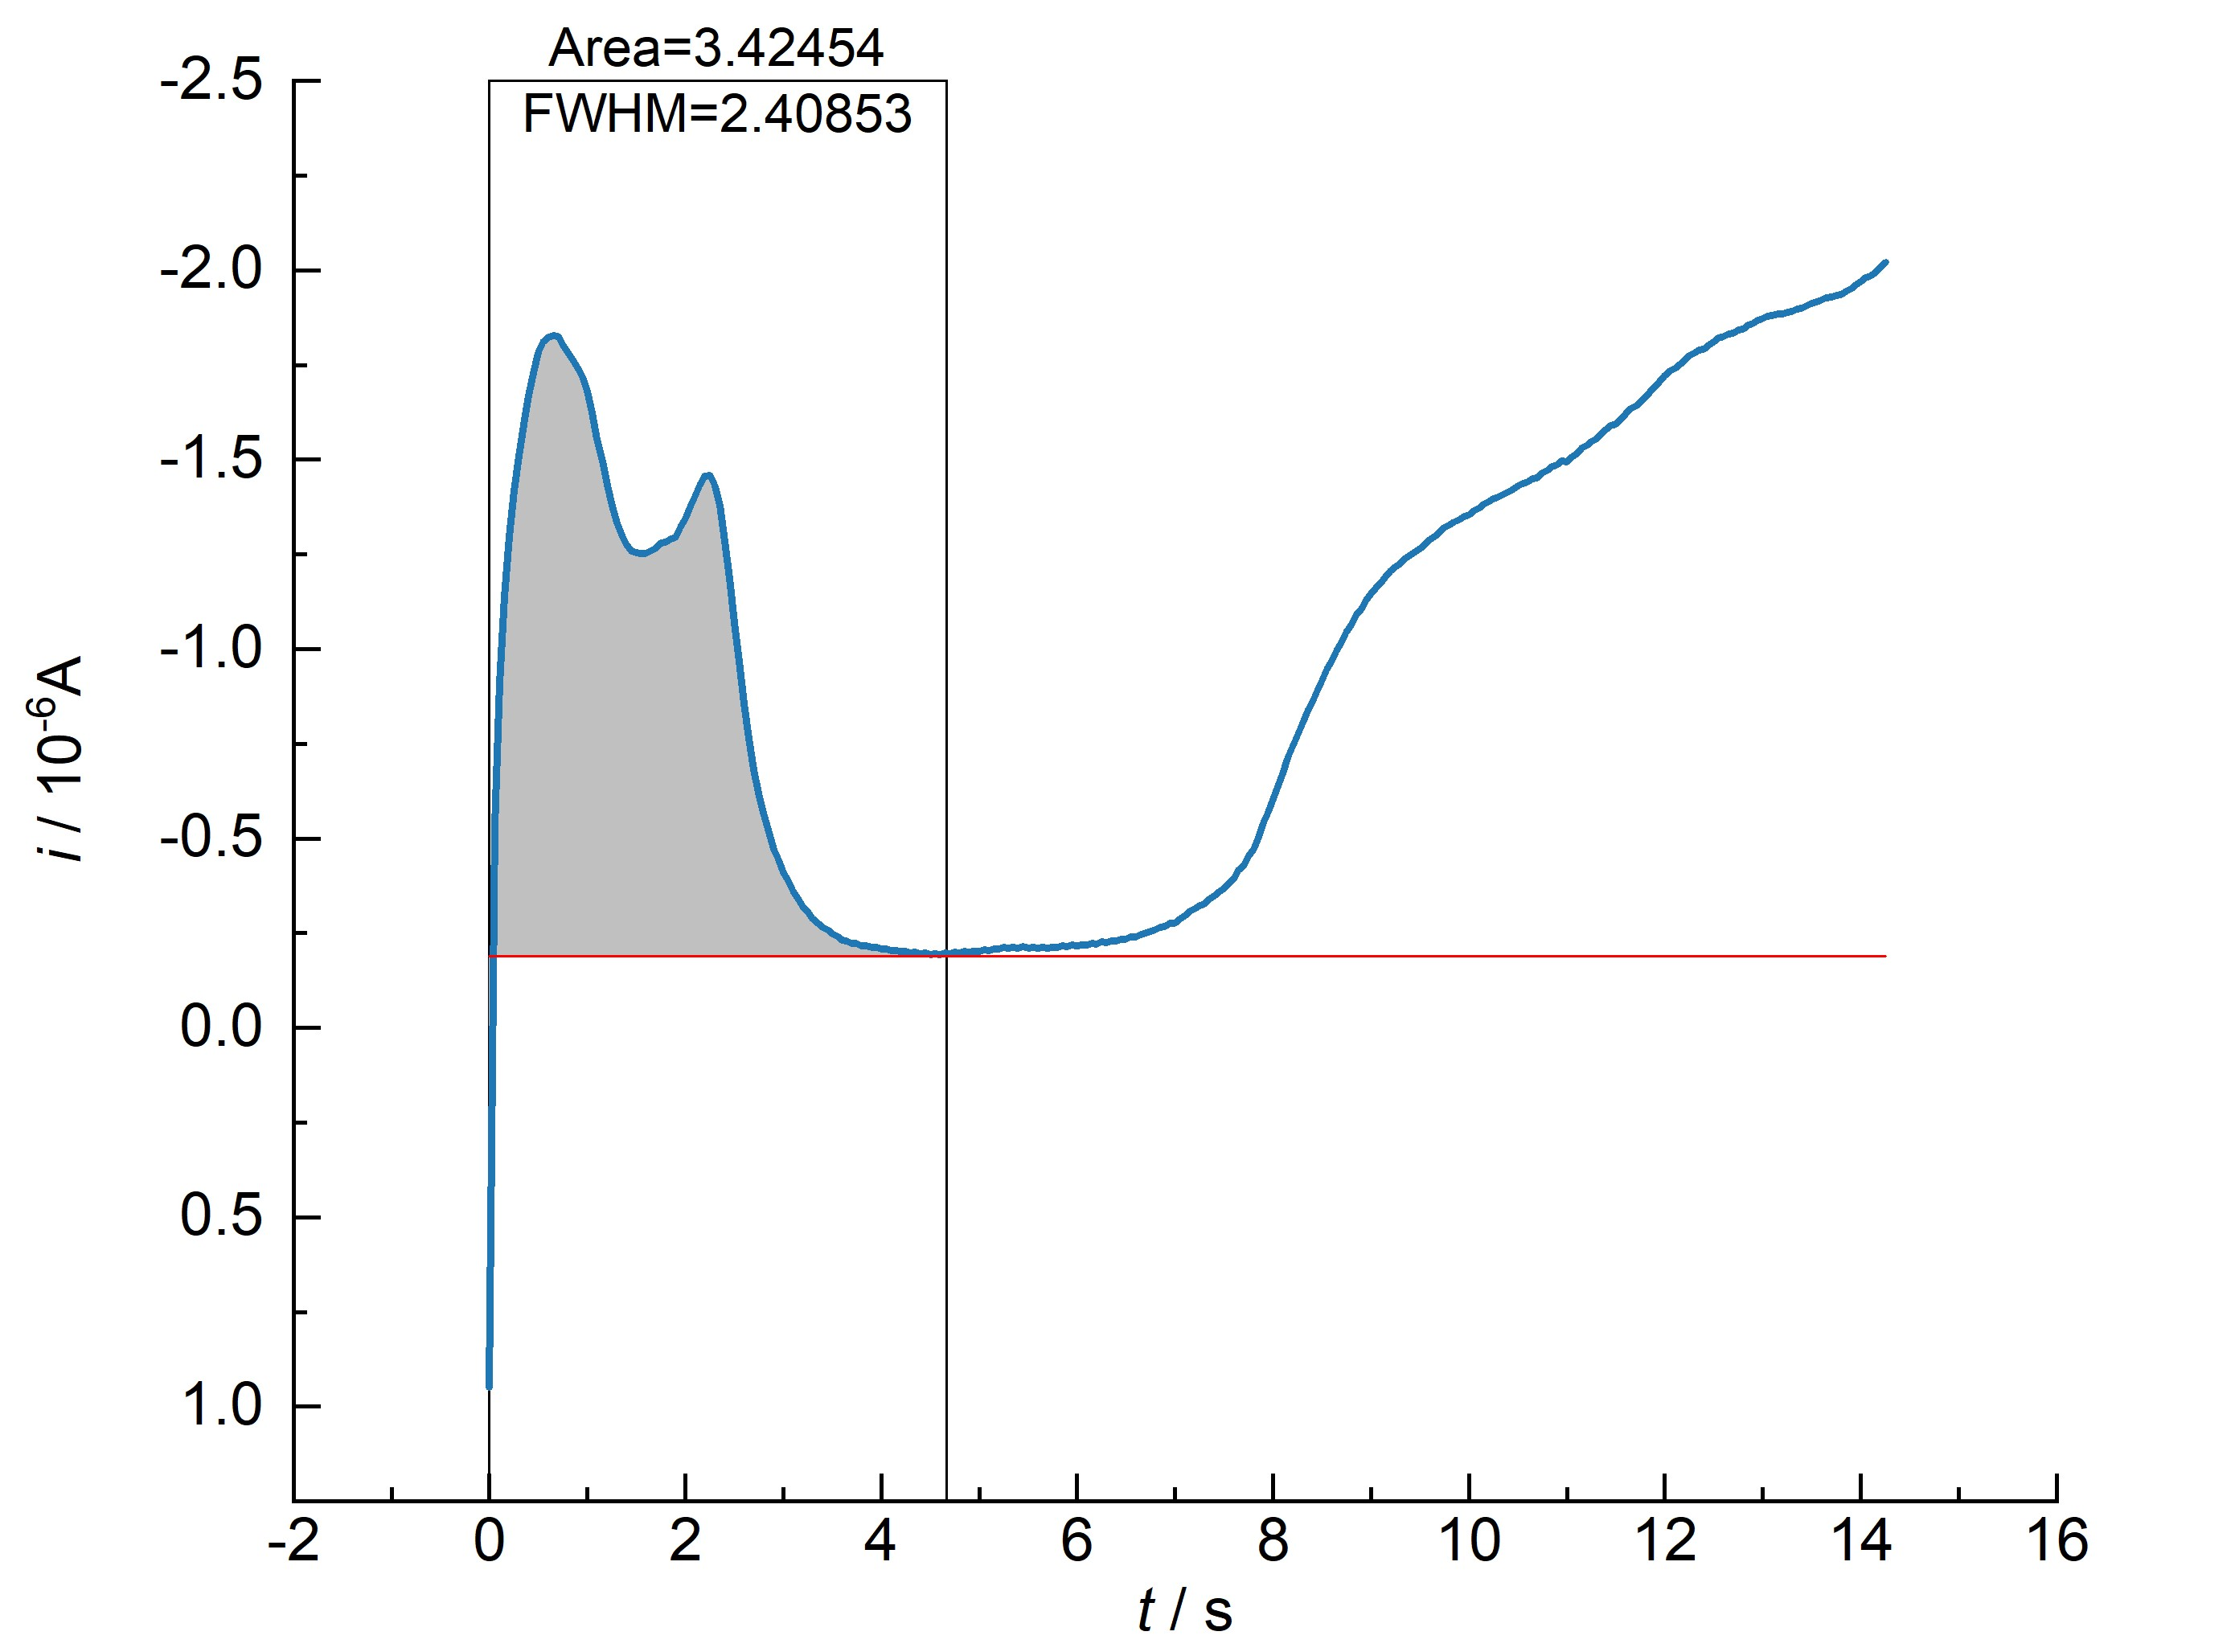
\includegraphics[width=0.65\textwidth]{5.jpg}
 	\bicaption{由铂电极CV曲线积分求氢原子脱附峰电量}{H desorption peak electricity calculation by integrating the CV curve of Pt electrode}
 \end{figure}
 \par
 根据\textbf{图5},读出铂电极表面单层氢原子脱附的电量
 $$
 q=3.42\times10^{-6}\ \ {\rm C}
 $$
 查阅资料\citealp{physchemlab}知多晶Pt表面满单层氢脱附的电量为$0.21\ \ {\rm mC\cdot m^{-2}}$,采用该数据进行计算,则实验使用的铂电极电化学活性面积
 $$
 S=\frac{3.42\times10^{-6}\ \ {\rm C}}{0.21\ \ {\rm mC\cdot cm^{-2}}}=1.6\times 10^{-2}\ \ {\rm cm^{2}}=0.016\ \ {\rm cm^{2}}
 $$
\subsubsection{直接甲醇燃料电池输出电压-输出功率曲线}
设定扫描速度为$0.1\ \ {\rm V\cdot s^{-1}}$,以${\rm N_{2}}$饱和的硫酸溶液中铂电极的CV曲线第10个segment的实验数据为背景,取电解质静止、${\rm O_{2}}$饱和的硫酸溶液中铂电极的CV曲线第10个segment的实验数据,扣除背景后,作为直接甲醇燃料电池Pt电极阴极$\rm O_{2}$还原的$\varphi-i$工作曲线;以${\rm N_{2}}$饱和的硫酸溶液中铂电极的CV曲线第9个segment的实验数据为背景,取硫酸溶液中铂电极表面MeOH电化学氧化反应的CV曲线第9个segment的实验数据,扣除背景后,作为直接甲醇燃料电池Pt电极阳极$\rm MeOH$氧化的$\varphi-i$工作曲线。两条$\varphi-i$曲线如\textbf{图6}所示。
 \begin{figure}[h]
	\centering
	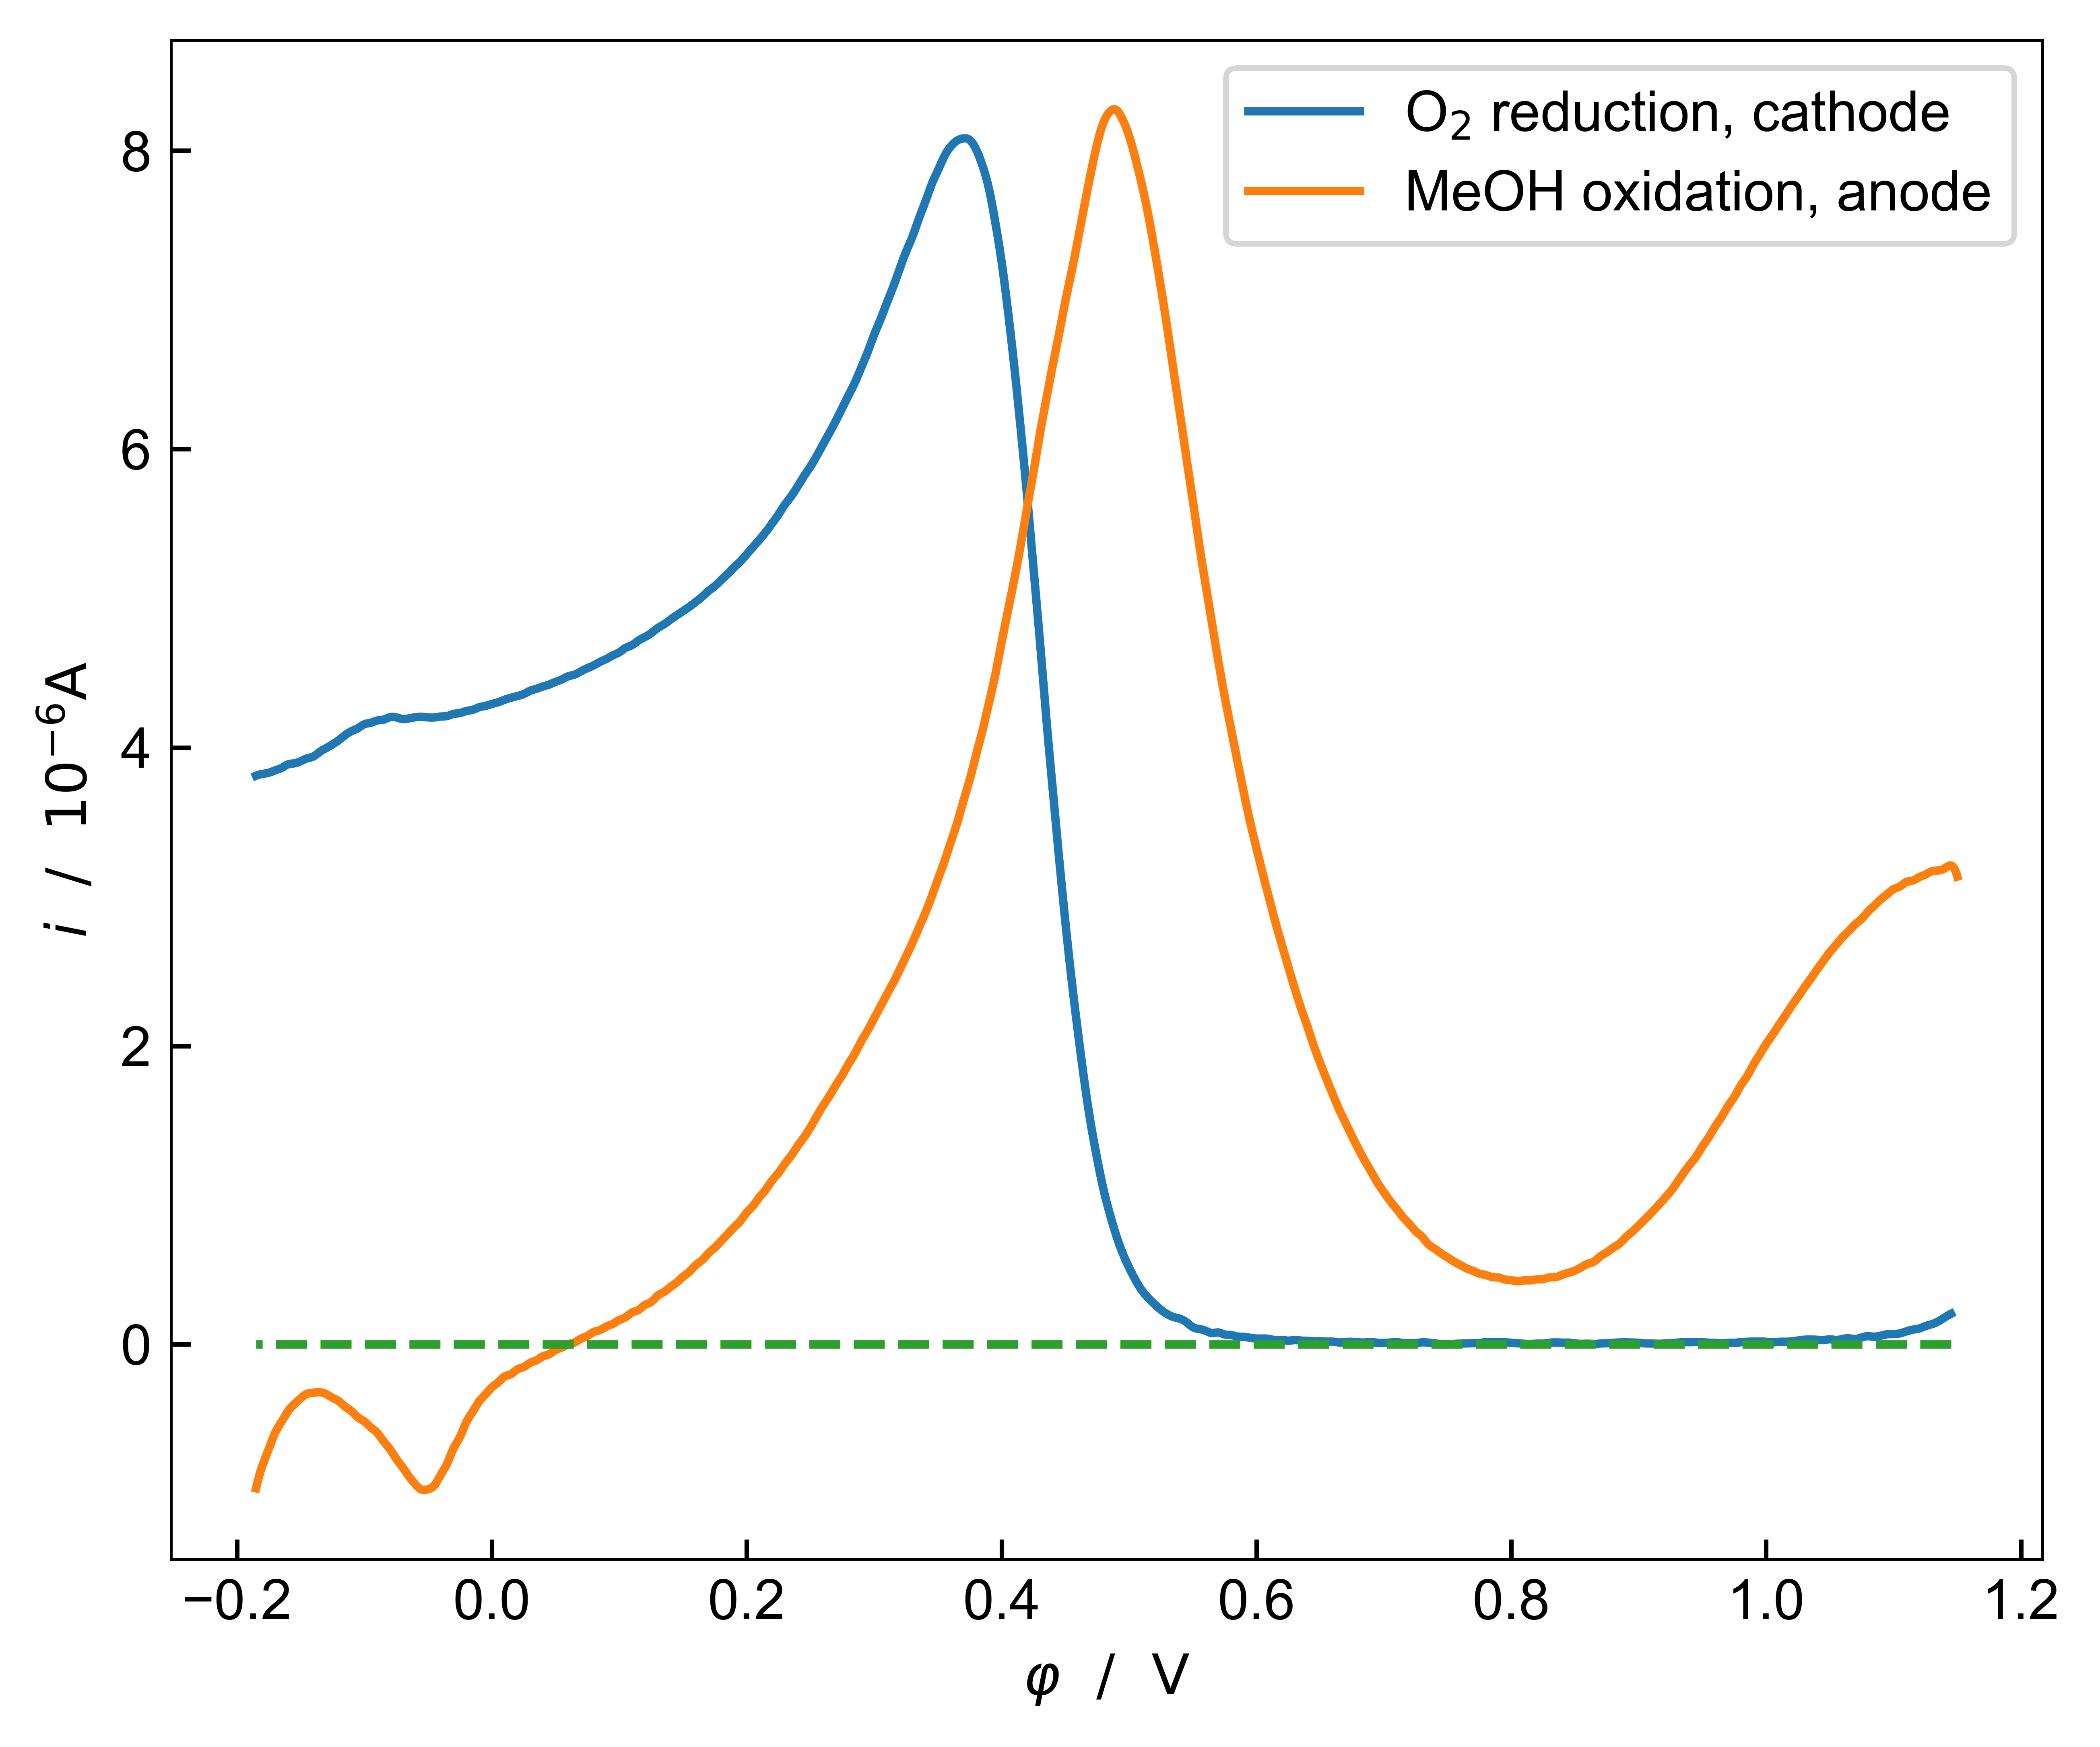
\includegraphics[width=0.65\textwidth]{6.jpg}
	\bicaption{直接甲醇燃料电池阳极、阴极$\varphi-i$工作曲线}{$\varphi-i$ working curve of anode and cathode of direct methanol fuel cell}
\end{figure}
\par
在直接甲醇燃料电池中,在一定的工作电流$i$下,阳极(负极,甲醇氧化)电势$\varphi_{a}$
低于阴极(正极,氧气还原)电势$\varphi_{c}$。在\textbf{图6}中选取$i$相同时$\varphi_{a}<\varphi_{c}$的部分,作一组平行于$\varphi$轴的直线与两条曲线相交,读取交点坐标对应的电势$\varphi_{a}$、$\varphi_{c}$,计算两极电势差
$$
U=\varphi_{c}-\varphi_{a}
$$
即为直接甲醇燃料电池的输出电压,根据
$$
P=Ui
$$
计算直接甲醇燃料电池的输出功率$P$。以上各项数据示于\textbf{表1}。
\begin{table}[h]
	\centering
	\zihao{5}
	\bicaption{直接甲醇燃料电池的两极电势、输出电压和输出功率}{Polar potential, output voltage and output power of direct methanol fuel cell}
	\begin{tabular}{ccccc}
		\toprule
		$i/{\rm 10^{-6}\ \ A}$ & $\varphi_{a}/{\rm V}$ & $\varphi_{c}/{\rm V}$ & $U/{\rm V}$ & $P/{\rm 10^{-6}\ \ W}$ \\
		\midrule
	0.01 & 0.064 & 0.682 & 0.618 & 0.006 \\
	0.50 & 0.156 & 0.501 & 0.345 & 0.173 \\
	1.00 & 0.212 & 0.481 & 0.269 & 0.269 \\
	1.50 & 0.253 & 0.471 & 0.218 & 0.327 \\
	2.00 & 0.288 & 0.461 & 0.173 & 0.346 \\
	2.50 & 0.320 & 0.454 & 0.134 & 0.335 \\
	3.00 & 0.344 & 0.449 & 0.105 & 0.315 \\
	3.50 & 0.366 & 0.442 & 0.076 & 0.266 \\
	4.00 & 0.381 & 0.438 & 0.057 & 0.228 \\
	4.50 & 0.396 & 0.432 & 0.036 & 0.162 \\
	5.00 & 0.407 & 0.427 & 0.020 & 0.100 \\
	5.30 & 0.414 & 0.424 & 0.010 & 0.053 \\
	5.50 & 0.418 & 0.422 & 0.004 & 0.022 \\
	5.58 & 0.419 & 0.421 & 0.002 & 0.011\\
		\bottomrule
	\end{tabular}
\end{table}
\par
根据\textbf{表1}数据,作出直接甲醇燃料电池的输出电压$U$-输出功率$P$曲线,如\textbf{图7}所示。
\begin{figure}[h]
	\centering
	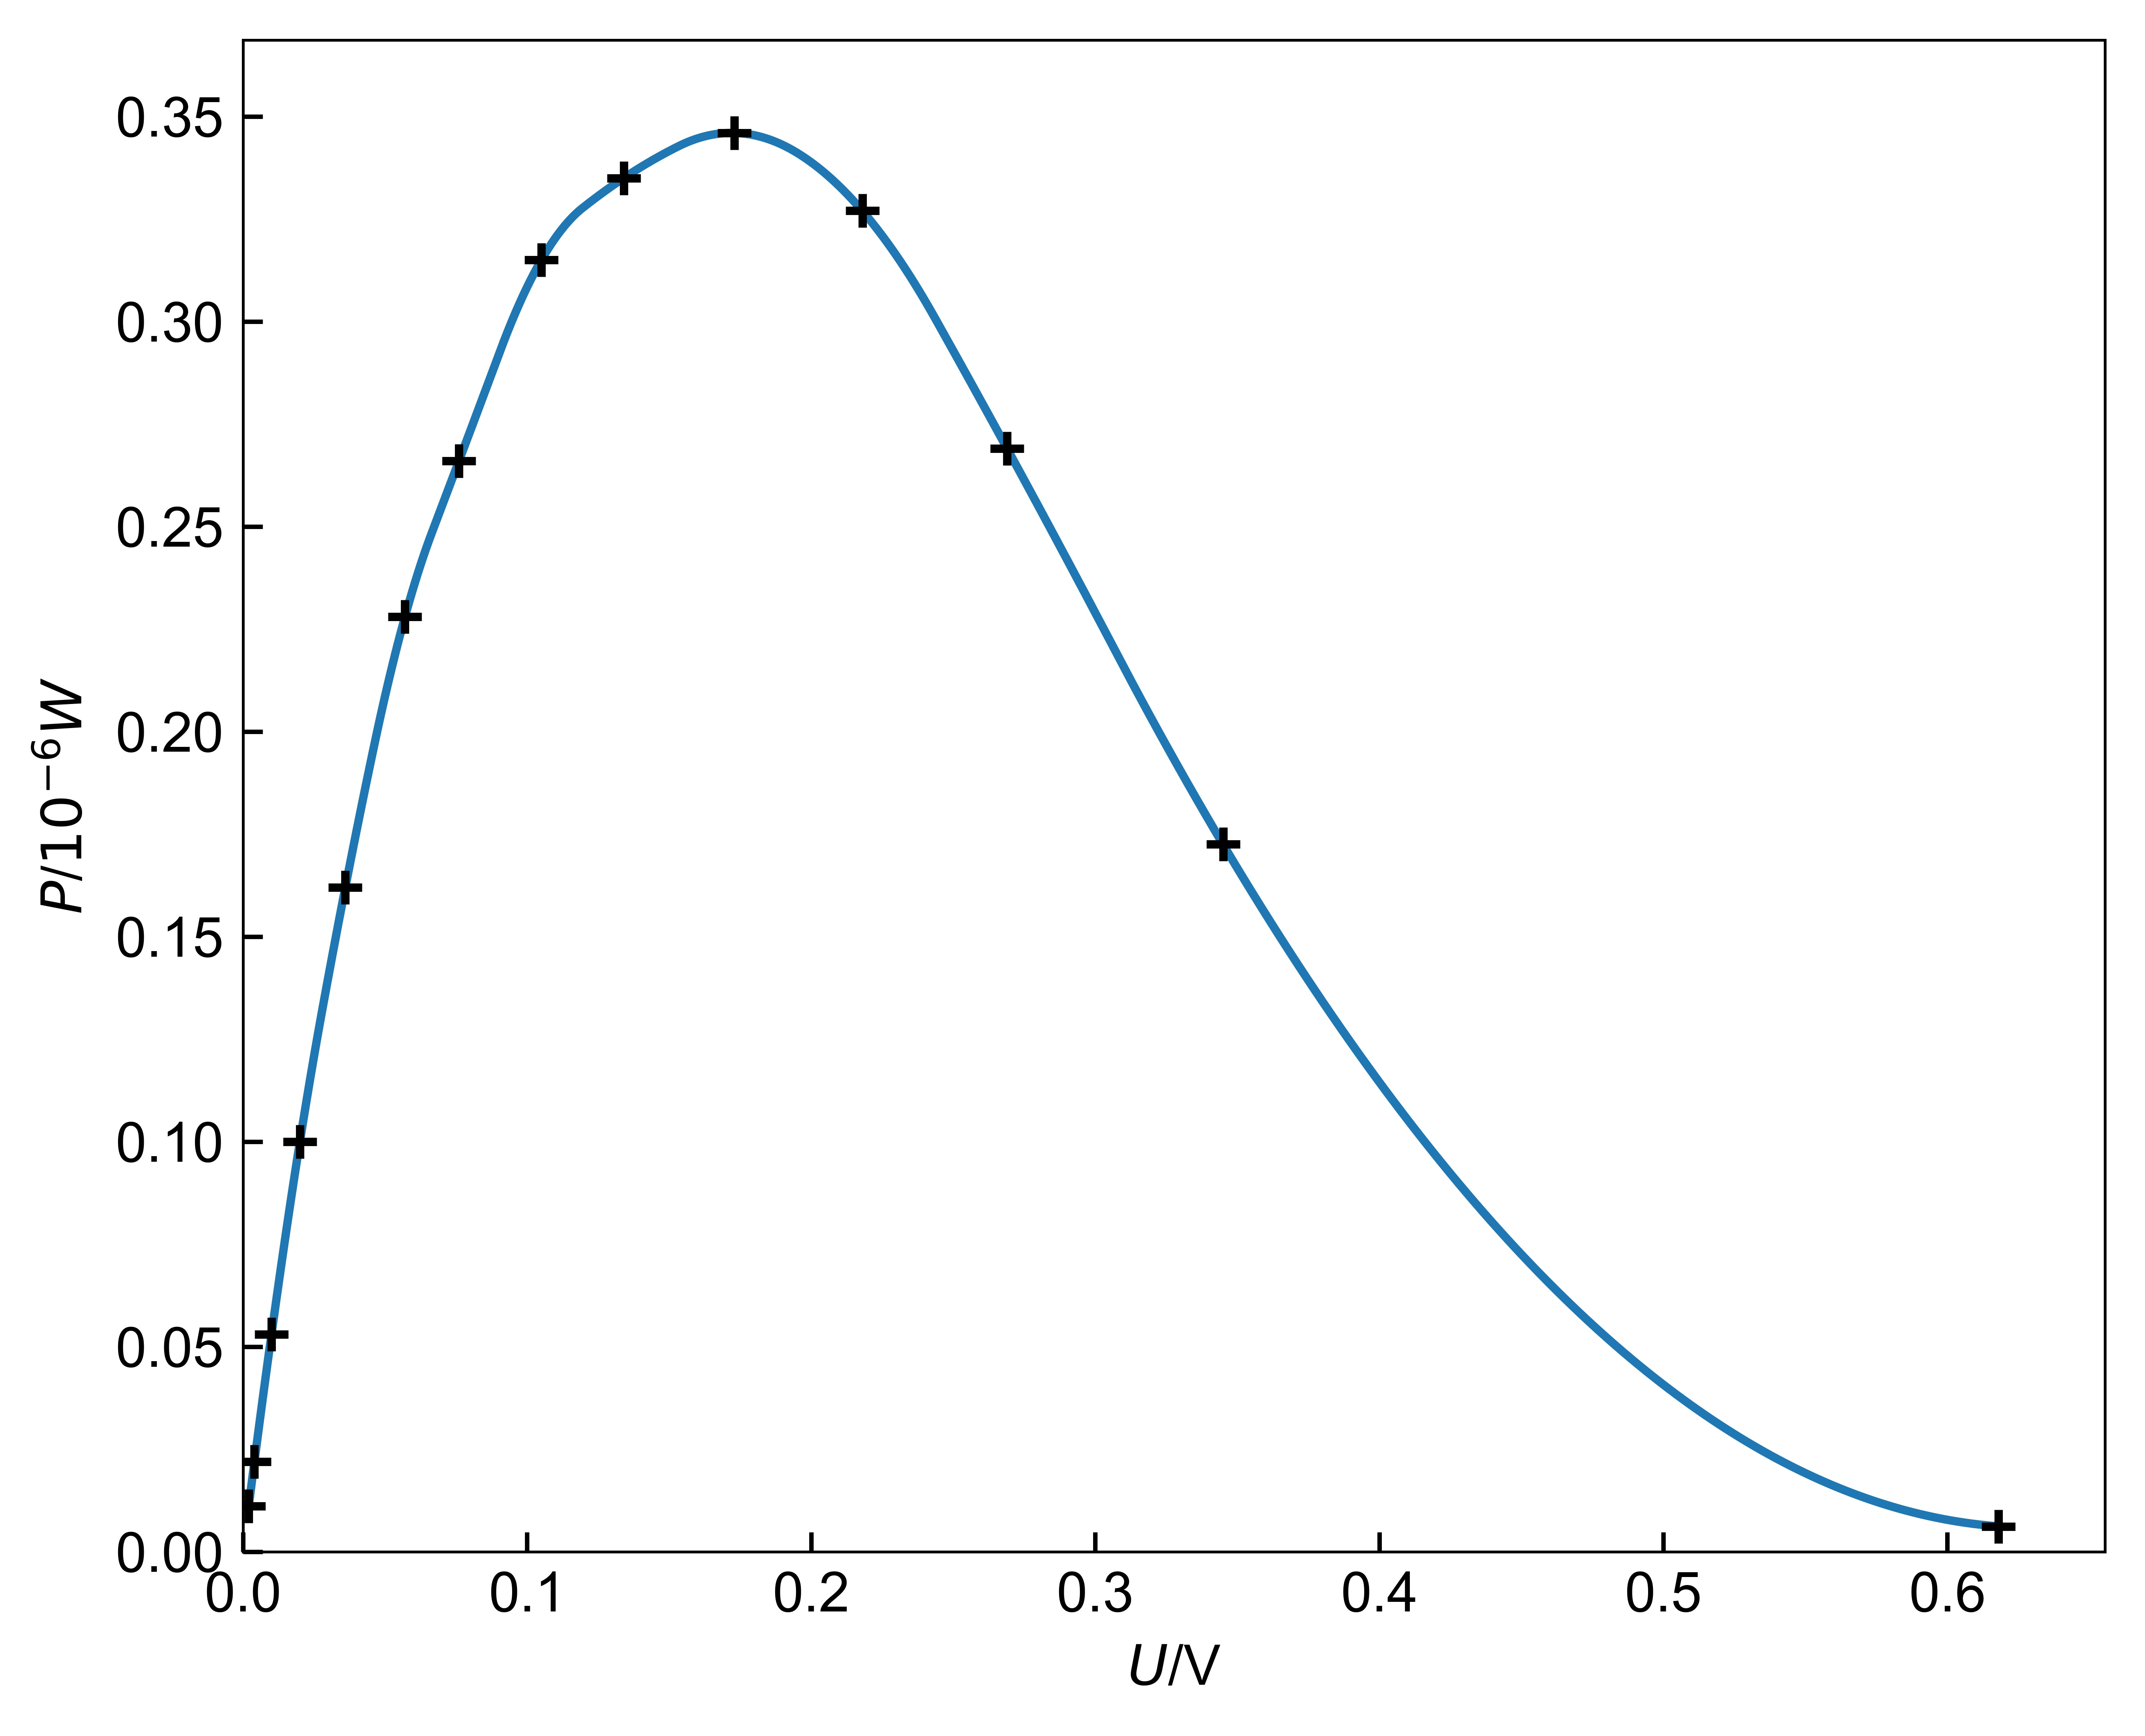
\includegraphics[width=0.587\textwidth]{7.jpg}
	\bicaption{直接甲醇燃料电池$U-P$曲线}{$U-P$ curve of direct methanol fuel cell}
\end{figure}
\par
根据\textbf{图7}可以看出,直接甲醇燃料电池的输出功率$P$随输出电压$U$的增大而先增大后减小,$U\approx0.2\ \ {\rm V}$时输出功率达最大值,$P_{max}\approx 3.5\times10^{-7}\ \ {\rm W}$。


 	 \section{讨论与结论}
		\subsection{实验讨论}
 			\subsubsection{测定铂电极电化学活性面积的误差分析}
利用氮气饱和的硫酸溶液中铂电极的CV曲线求算铂电极电化学活性面积时,可能的误差来源分析如下。\par 
第一,在实际选择的电位窗口内,在进行循环扫描的过程中,氢的吸附和脱附过程可能进行不完全,由于选择的最低电位仍然太高,氢尚未充分吸附到铂电极表面时,扫描已经反向,开始脱附过程,导致氢原子未能充分占据铂电极表面的全部活性位点,测算的铂电极电化学活性面积偏小。\par 
第二,由于电极极化,氢原子脱附的实际电量与根据CV曲线测算的电量并不严格相等,有一部分电子转移过程中的电量损耗,CV曲线积分得到的电量大于实际氢原子脱附的电量,导致测算的铂电极电化学活性面积偏大。\par 
以上两个原因可能导致铂电极电化学活性面积的测定不够准确。
\subsubsection{直接甲醇燃料电池$U-P$曲线的误差分析}
根据铂电极表面氧还原反应和甲醇电化学氧化反应的CV曲线绘制直接甲醇燃料电池的$U-P$工作曲线时,可能的误差来源分析如下。\par 
甲醇电化学氧化的CV曲线测定不够准确,根据\textbf{图4}可以看出,甲醇氧化的双电层区有一定程度的上抬,在氢区与$\rm N_{2}$的曲线不重合,导致在扣除背景时出现一定的偏差,从而导致甲醇氧化的CV曲线不够准确。
 	 	\subsubsection{实验改进}
在实际实验中,需要仔细调节所选择的电位窗口,可以在不出现水的还原峰的情况下尽可能取较低的最低电位,从而能够减小测定铂电极电化学活性面积的实验误差。


 	 \subsection{实验结论}
本实验使用三电极电解池研究铂圆盘电极表面的电化学反应,调整合适的电位窗口,用${\rm N_{2}}$饱和的${\rm 0.05 \ \ M}$硫酸对电极系统进行活化,测定了扫描速度为$0.5$、$0.2$和$0.1\ \ {\rm V\cdot s^{-1}}$时的CV曲线,对比三条曲线,得到了峰电流随扫描速度变大而变大的结论。对CV曲线进行积分,得到铂电极表面单层氢原子吸附的电量$q=3.42\times 10^{-6}\ \ {\rm C}$,铂电极电化学活性面积$S=0.016\ \ {\rm cm^{2}}$。测定了不同搅拌速度下铂电极表面氧还原反应的CV曲线,分析了造成曲线形态不同的原因,读出氧气的起始还原电位$0.57\ \ {\rm V}$。测定铂电极表面甲醇氧化反应的CV曲线,读出甲醇的起始氧化电位$0.06\ \ {\rm V}$。根据铂电极表面氧还原反应和甲醇电化学氧化反应的CV曲线,绘制了直接甲醇燃料电池的$U-P$工作曲线,从曲线中读出工作电压为$0.2\ \ {\rm V}$时,达到最大输出功率$3.5\times 10^{-7}\ \ {\rm W}$。


 

   

\vbox{}

\bibliographystyle{achemso}
\bibliography{cite}



\end{document}